\section*{Aufgabe 2 (24 Punkte)}
\vspace{0.4cm}
\subsection*{\aufgabe{a1}{5}}
Sei $ a_k = \ln \left( 1 + \left( \frac{1}{2}\right)^k \right) $ für $ k = 1,2,... $\\
\\
Verwenden Sie das Taylorpolynom $ P_2 $ zweiter Ordnung der Funktion
\begin{align*}
f \ : \ D_f \to \mathbb{R}, \ x \mapsto y = f(x) = \ln(1+x)
\end{align*}
im Punkt $ x_0 = 0 $, um einen Näherungswert für 
$ \sum_{k=1}^\infty a_k $ zu bestimmen.
\\
\\
\textbf{Lösung:}
\begin{mdframed}
\renewcommand{\labelenumi}{\theenumi.}
\underline{\textbf{Vorgehensweise:}}
\begin{enumerate}
\item Bestimme allgemein das Taylorpolynom zweiter Ordnung an $ P_2 $.
\item Berechne $ P_2 $.
\item Approximiere die Reihe.
\end{enumerate}
\end{mdframed}

\underline{1. Bestimme allgemein das Taylorpolynom $ P_2 $ zweiter Ordnung an}\\
Im Allgemeinen berechnen wir das $ n $-te Taylorpolynom im Entwicklungspunkt $ x_0 $ durch
\begin{align*}
P_n(x) = \sum \limits_{k=0}^n \frac{f^{k}(x_0)}{k!} (x-x_0)^k.
\end{align*}
Allgemein müssen wir in unserem Fall wegen $ x_0 = 0 $
\begin{align*}
P_2(x) 
%= f(x_0 ) + f^\prime(x_0) (x - x_0) + \frac{f^{\prime \prime}(x_0)}{2}(x - x_0)^2
= 
f(0) + f^{\prime}(0) x + \frac{f^{\prime \prime}(0)}{2} x^2
\end{align*}
berechnen.
\\
\\
\underline{2. Berechne $ P_2 $}\\
Wir bestimmen zunächst mithilfe der Kettenregel die Ableitungen.
Es gilt
\begin{align*}
f(x) &= \ln(1+x)\\
f^\prime(x) &= \frac{1}{1+ x} = (1+x)^{-1}\\
f^{\prime \prime}(x) &=-1 \cdot (1+x)^{-2} = - \frac{1}{(1+x)^2}
\end{align*}
womit 
\begin{align*}
f(0) &= 0 \\
f^\prime(0) &= 1\\
f^{\prime \prime}(0 ) &= -1
\end{align*}
folgt.
Damit erhalten wir 
\begin{align*}
P_2(x) = x - \frac{x^2}{2}.
\end{align*}

\underline{3. Approximiere die Reihe}\\
Nun ist $ P_2 $ eine Approximation unserer Funktion $ f $, daher gilt
\begin{align*}
a_k = \ln \left( 1 + \left( \frac{1}{2}\right)^k \right)
\approx P_2 \left( \left( \frac{1}{2}\right)^k\right)
= 
\left(\frac{1}{2}\right)^k - \frac{1}{2} \left(\left(\frac{1}{2}\right)^k \right)^2
=
\left(\frac{1}{2}\right)^k - \frac{1}{2} \left(\frac{1}{4}\right)^k. 
\end{align*} 
Unter Verwendung der geometrischen Reihe erhalten wir eine Approximation der Reihe:
\begin{align*}
\sum \limits_{k=1}^\infty a_k
&\approx 
\sum \limits_{k=1}^\infty
\left(\left(\frac{1}{2}\right)^k - \frac{1}{2} \left(\frac{1}{4}\right)^k\right)
= 
\sum \limits_{k=1}^\infty \left(\frac{1}{2}\right)^k
- \frac{1}{2} \sum \limits_{k=1}^\infty \left(\frac{1}{4}\right)^k
=
\frac{1}{2} \sum \limits_{k=0}^\infty \left(\frac{1}{2}\right)^k
\frac{1}{2\cdot 4} \sum \limits_{k=0}^\infty \left(\frac{1}{4}\right)^k\\
&=\frac{1}{2} \frac{1}{1 - \frac{1}{2}} - \frac{1}{8} \frac{1}{1 - \frac{1}{4}}
= \frac{1}{2} \cdot 2 - \frac{1}{8} \frac{4}{3}
= 1 - \frac{1}{6} = \frac{5}{6}.
\end{align*}      
\newpage          
                  
\subsection*{\aufgabe{a2}{4}}
Gegeben ist die Funktion
\begin{align*}
f \ : \ D_f \to \mathbb{R}, \ x \mapsto y = f(x) = \ln(1+x).
\end{align*}
$ R_2 $ bezeichne das Restglied zweiter Ordnung von $ f  $ in $ x_0 = 0 $.\\
\\
Zeigen Sie
\begin{align*}
\sum \limits_{k=1}^\infty R_2 \left( \left( \frac{1}{2}\right)^k \right) \leq \frac{1}{21}.
\end{align*}
\\
\textbf{Lösung:}
\begin{mdframed}
\underline{\textbf{Vorgehensweise:}}
\begin{enumerate}
\renewcommand{\labelenumi}{\theenumi.}
\item Gebe die allgemeine Formel für das Restglied an.
\item Forme das Restglied um.
\item Zeige die Ungleichung.
\end{enumerate}
\end{mdframed}

\underline{1. Gebe die allgemeine Formel für das Restglied an}\\
Das Restglied $ n $-ter Ordnung für $ f $ im Punkt $ x_0 $ ist durch
\begin{align*}
R_n(x) = \frac{f^{n+1}(\xi)}{(n+1)!}(x - x_0)^{(n+1)} 
\end{align*}
für $ \xi \in [x_0,x] $ gegeben. Für unseren Fall ergibt sich also
\begin{align*}
R_2(x) = \frac{f^{(3)}(\xi)}{3!} x^3
\end{align*}
für $ \xi \in [0,x] $.
\\
\\

\underline{2. Forme das Restglied um}\\
Aus der letzten Aufgabe erhalten wir
\begin{align*}
f^{\prime \prime}(x) = - \frac{1}{(1+x)^2}
\
\Rightarrow
\
f^{(3)}(x) = \frac{2}{(1+x)^3}
\end{align*}
und damit gilt
\begin{align*}
R_2(x) = \frac{f^{(3)}(\xi)}{3!} x^3 = \frac{1}{6} \frac{2}{(1+\xi)^3} x^3
=
\frac{1}{3} \frac{1}{(1+\xi)^3} x^3
\Rightarrow
R_2(x) = \frac{1}{3} \underbrace{\frac{1}{(1+\xi)^3}}_{\leq 1} x^3
\leq 
\frac{x^3}{3}
\end{align*}
für $ x \in [0,1] $.
\\

\underline{3. Zeige die Ungleichung}\\
Mit unseren Überlegungen erhalten wir durch
\begin{align*}
\sum \limits_{k=1}^\infty R_2 \left( \left( \frac{1}{2}\right)^k \right)
\leq 
\sum \limits_{k=1}^\infty \frac{1}{3} \left( \frac{1}{2}\right)^{3k}
=
\frac{1}{3} \sum \limits_{k=1}^\infty  \left( \frac{1}{8}\right)^{k}
=
\frac{1}{3 \cdot 8} 
\sum \limits_{k=0}^\infty  \left( \frac{1}{8}\right)^{k}
=
\frac{1}{24} \cdot \frac{1}{1 - \frac{1}{8}}
=
\frac{1}{24} \cdot \frac{8}{7} = \frac{1}{21}
\end{align*} 
die gesuchte Ungleichung.


\subsection*{\aufgabe{b}{4}}
Gegeben ist die Funktion 
\begin{align*}
f(x,y)
=
\frac{\ln(9 - 9 x^2 - y^2)}{(x-y) \sqrt{4 - x^2 - y^2}}.
\end{align*}

Ermitteln Sie den Definitionsbereich $ D_f $ von $ f $ und stellen Sie diesen graphisch dar.
\\
\\

\textbf{Lösung:}
\begin{mdframed}
\underline{\textbf{Vorgehensweise:}}
\renewcommand{\labelenumi}{\theenumi.}
\begin{enumerate}
\item Überlege dir, für welche Werte die Funktion definiert ist.
\item Gebe den Definitionsbereich graphisch an.
\end{enumerate}
\end{mdframed}

\underline{1. Überlege dir, für welche Werte die Funktion definiert ist}\\
Wir betrachten zunächst den Zähler $ \ln(9 - 9 x^2 - y^2) $. 
Dieser ist definiert, falls der Ausdruck im Logarithmus größer Null ist. Daher muss
\begin{align*}
9 - 9x^2 -y^2  > 0 
\ 
\Leftrightarrow \
9 > 9x^2 + y^2
\
\Leftrightarrow
\
1 > x^2 + \frac{y^2}{9} = x^2 + \frac{y^2}{3^2}
\end{align*}
gelten. Die Gleichung
\begin{align*}
x^2  + \frac{y^2}{3^2} < 1
\end{align*}
beschreibt die Fläche innerhalb einer Ellipse mit Mittelpunkt $ (0,0) $ und den Halbachsen $ a = 1 $ und $ b = 3 $.
Nun betrachten wir den Nenner $ (x-y) \sqrt{4 - x^2 - y^2} $. Zunächst muss $ x \neq y $ gelten. 
Für die Wurzel muss noch
\begin{align*}
4 -x^2 - y^2 > 0
\
\Leftrightarrow
\
x^2 + y^2 < 4 = 2^2
\end{align*}
erfüllt sein.
Beachte, dass die Wurzelfunktion definiert ist, falls der enthaltene Ausdruck größer gleich Null ist.
Da die Wurzel im Nenner steht, müssen wir den gleich Null Fall ausschließen.
Hierdurch wird eine Kreisfläche mit Mittelpunkt $ (0,0) $ und Radius $ 2 $ beschrieben.
\\
\\
\underline{2. Gebe den Definitionsbereich graphisch an}\\
Zusammengefasst erhalten wir die drei Bedingungen
\begin{align*}
x \in D_f \
\Leftrightarrow
\
\begin{cases}
x \neq y\\
x^2  + \frac{y^2}{3^2} < 1\\
x^2 + y^2 <  2^2.
\end{cases}
\end{align*}
Diese lassen sich durch die Skizze
\begin{center}
%	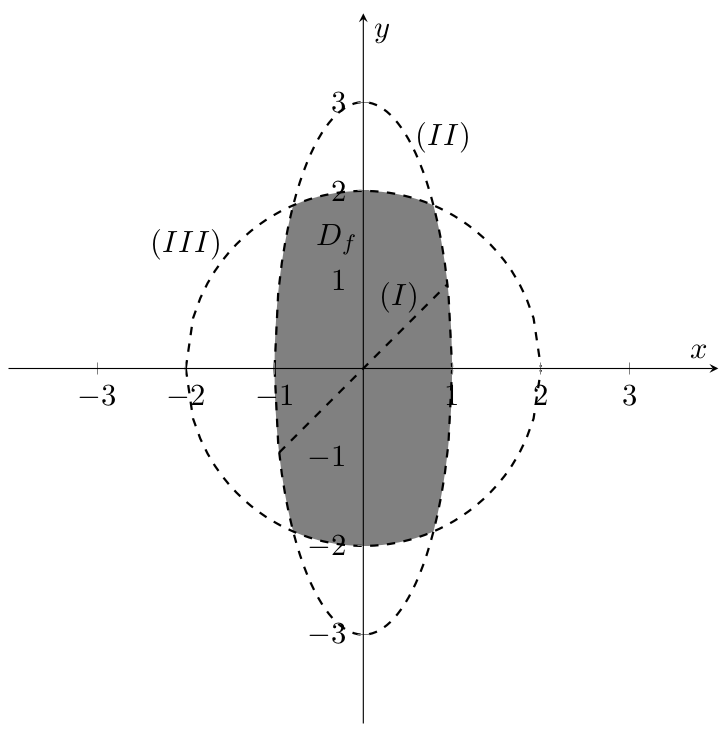
\includegraphics[width=0.5\textwidth]{pictures/auf2_b.png}
\end{center}
veranschaulichen.

\newpage
\subsection*{\aufgabe{c}{5}}
Gegeben sei die Nutzenfunktion
\begin{align*}
u(c_1,c_2) = c_1^\alpha c_2^{1-\alpha}
\end{align*}
für $ \alpha \in (0,1) $, wobei $ c_1,c_2 $ die konsumierten Mengen der Güter 1 und 2 sind, und die Budgetrestriktion
\begin{align*}
C \ : \ p_1 c_1 + p_2 c_2 = 10
\end{align*}
für Preise $ p_1 > 0  $ und $ p_2 > 0 $.\\
\\
Für welche Werte der Parameter $ \alpha, p_1, p_2 $ berührt die Niveaulinie (Indifferenzkurve) $ u(c_1,c_2) = \sqrt{2} $ die Budgetlinie $ C $ im Konsumgüterbündel $ (c_1^\star,c_2^\star)  = (1,2)$?
\\
\\
\textbf{Lösung:}
\begin{mdframed}
\underline{\textbf{Vorgehensweise:}}
\renewcommand{\labelenumi}{\theenumi.}
\begin{enumerate}
\item Gebe die mathematische Formulierung des Problems an.
\item Wende das Theorem für implizite Funktionen an, um das Problem zu lösen.
\end{enumerate}
\end{mdframed}

\underline{1. Gebe die mathematische Formulierung des Problems an}\\
Das Konsumgüterbündel $ (c_1^\star,c_2^\star)  = (1,2)$ eingesetzt in die Budgetrestriktion ergibt die Budgetgerade
\begin{align*}
 p_1 + 2 p_2 = 10
 \
 \Leftrightarrow
 \
 p_1 = 10 - 2 p_2.
\end{align*}
Weiter muss wegen
\begin{align*}
u(1,2) = 1^\alpha 2^{1-\alpha} = \sqrt{2}
\end{align*}
$ \alpha = 0.5 $ gelten.
Die letzte Bedingung ist, dass sich die beiden Kurven 
\begin{align*}
u(c_1,c_2) = \sqrt{2 } 
 \ \Leftrightarrow \ 
f(c_1,c_2) &:= u(c_1,c_2) - \sqrt{2} = c_1^{0.5}c_2^{0.5} - \sqrt{2} =  0\\
p_1 c_1 + p_2 c_2 = 10
\ \Leftrightarrow \
\varphi(c_1,c_2) &:= p_1 c_1 + p_2 c_2 - 10 = 0
\end{align*}
in $ (c_1^\star,c_2^\star)  = (1,2)$ berühren.
\\
\\
\underline{2. Wende das Theorem für implizite Funktionen an, um das Problem zu lösen}\\ 
Das Theorem für implizite Funktionen liefert uns den Zusammenhang
\begin{align*}
- \frac{f_{c_1}(1,2)}{f_{c_2}(1,2)}
=
- \frac{\varphi_{c_1}(1,2)}{\varphi_{c_2}(1,2)}
\end{align*}
und es gelten 
\begin{align*}
f_{c_1}(c_1,c_2) = 0.5 c_1^{-0.5} c_2^{0.5}
&\Rightarrow 
f_{c_1}(1,2) = 0.5 \sqrt{2}\\
f_{c_2}(c_1,c_2) = 0.5 c_1^{0.5} c_2^{-0.5}
&\Rightarrow 
f_{c_1}(1,2) = 0.5 \frac{1}{\sqrt{2}}\\
\varphi_{c_1}(1,2) = p_1, &\qquad 
\varphi_{c_2}(1,2) = p_2.
\end{align*}
Insgesamt erhalten wir die Gleichung
\begin{align*}
- \frac{0.5 \sqrt{2}}{0.5 \frac{1}{\sqrt{2}}} = - \frac{p_1}{p_2}
\
\Leftrightarrow
\
2 p_2 = p_1
\end{align*}
und mit $ p_1 = 10 - 2 p_2 $ folgt
\begin{align*}
2 p_2 = 10 - 2 p_2 \ 
\Leftrightarrow
\
4 p_2 = 10 
\ \Leftrightarrow \
p_2 = \frac{10}{4} = \frac{5}{2} = 2.5.
\end{align*}
Wegen $ p_1 = 2 p_2 $ gilt dann auch $ p_2 = 2 \cdot 2.5 = 5 $.
Das Endresultat ist also durch
\begin{align*}
\alpha = 0.5 , \ p_1 = 5, \ p_2 =  \frac{5}{2}
\end{align*}
gegeben.

\newpage


\subsection*{\aufgabe{d}{6}}
Die Funktionen $ f $ und $ g $ sind auf $ \mathbb{R}^2_{++} $ definiert und haben den Wertebereich $ \mathbb{R}_{++} $.
Außerdem ist die Funktion $ f $ homogen vom Grad $ r $ und die Funktion $ g $ homogen vom Grad $ r -2 $.\\
Für die Funktion $ h $ gilt:
\begin{align*}
h(x,y) &= \frac{f(x,y)}{g(x,y)}\\
h_y(x,y) &= x  - \frac{3}{2} x^{0.5} y^{0.5}
\end{align*}
und
\begin{align*}
\varepsilon_{h,x}(x,y)
= 
\frac{xy - \frac{1}{2}x^{0.5} y^{1.5}}{xy - x^{0.5} y^{1.5}}
\end{align*}
Ermitteln Sie $ h(x,y) $ und vereinfachen Sie den Funktionsterm.
\\
\\
\textbf{Lösung:}
\begin{mdframed}
\underline{\textbf{Vorgehensweise:}}
\renewcommand{\labelenumi}{\theenumi.}
\begin{enumerate}
\item Überlege dir, was du aus der Homogenität von $ f $ und $ g $ schließen kannst.
\item Verwende das Resultat, um die Aufgabe zu lösen.
\end{enumerate}
\end{mdframed}

\underline{1. Überlege dir, was du aus der Homogenität von $ f $ und $ g $ schließen kannst}\\
Nach Voraussetzung ist $ f $ homogen vom Grad $ r $ und $ g $ homogen vom Grad $ r-2 $, d.h.
\begin{align*}
f(\lambda x , \lambda y) &= \lambda^r f(x,y)\\
g(\lambda x , \lambda y) &= \lambda^{r-2} g(x,y).
\end{align*}
Dies liefert uns mit
\begin{align*}
h(\lambda x , \lambda y)
= 
\frac{f(\lambda x , \lambda y)}{g(\lambda x , \lambda y)}
=
\frac{\lambda^{r} f(x,y)}{\lambda^{r-2} g(x,y)}
=
\lambda^2 \frac{f(x,y)}{g(x,y)}
=
\lambda^2 h(x,y)
\end{align*}
die Homogenität vom Grad $ 2 $ für $ h $.
Wir betrachten die partielle Elastizität
\begin{align*}
\varepsilon_{h,x}(x,y) = x \frac{h_x(x,y)}{h(x,y)}
\
\Leftrightarrow
\
\varepsilon_{h,x}(x,y) h(x,y) = x h_x(x,y)
\end{align*}
und die eulerschen Relation
\begin{align*}
x h_x(x,y) + y h_y(x,y) = 2 h(x,y).
\end{align*}
Die Kombination beider Aussagen liefert
\begin{align*}
&\quad \ \ \varepsilon_{h,x}(x,y) h(x,y) + y h_y(x,y) = 2 h(x,y)\\
&\Leftrightarrow
y h_y(x,y) = 2 h(x,y)- \varepsilon_{h,x}(x,y) h(x,y) =
h(x,y) ( 2 - \varepsilon_{h,x}(x,y)) \\
&\Leftrightarrow
h(x,y) = \frac{y h_y(x,y)}{2 - \varepsilon_{h,x}(x,y)} 
\end{align*}
wodurch wir eine Darstellung für $ h $ gefunden haben.
Durch Einsetzen von $ h_y $ und $ \varepsilon_{h,x} $ erhalten wir nun die Lösung.
\\
\\
\underline{2. Verwende das Resultat, um die Aufgabe zu lösen}\\
Es gilt
\begin{align*}
h(x,y) &= \frac{y h_y(x,y)}{2 - \varepsilon_{h,x}(x,y)} 
=
\frac{y \left( x  - \frac{3}{2} x^{0.5} y^{0.5} \right)}{2 -  
	\frac{xy - \frac{1}{2}x^{0.5} y^{1.5}}{xy - x^{0.5} y^{1.5}}
	}
=
\frac{y \left( x  - \frac{3}{2} x^{0.5} y^{0.5} \right)}
{\frac{2 (xy - x^{0.5} y^{1.5})}{xy - x^{0.5} y^{1.5}} -  
	\frac{xy - \frac{1}{2}x^{0.5} y^{1.5}}{xy - x^{0.5} y^{1.5}}
}\\
&=
\frac{y \left( x  - \frac{3}{2} x^{0.5} y^{0.5} \right)}
{2 (xy - x^{0.5} y^{1.5}) -  
	xy + \frac{1}{2}x^{0.5} y^{1.5}
}
(xy - x^{0.5} y^{1.5})
=
\frac{  xy  - \frac{3}{2} x^{0.5} y^{1.5} }
{xy  -  
	 \frac{3}{2}x^{0.5} y^{1.5}
}
(xy - x^{0.5} y^{1.5})\\
&=
xy - x^{0.5} y^{1.5}, 
\end{align*}
womit 
\begin{align*}
h(x,y) = xy - x^{0.5} y^{1.5}
\end{align*}
folgt.